\section{Estatística Bayesiana Computacional}

Até o momento, trabalhamos com modelos tais que
era possível calcular analiticamente 
a distribuição a posteriori para o parâmetro do
modelo estatístico. Para tal, usamos a expressão
obtida a partir do Teorema de Bayes:
\begin{align*}
 f(\theta|x)
 &= \frac{f(\theta)f(x|\theta)}
 {\int{f(\theta)f(x|\theta)d\theta}}
\end{align*}

Contudo, geralmente não é possível calcular diretamente
$\int{f(\theta)f(x|\theta)d\theta}$
ou aproximar esta expressão por métodos determinísticos de
integração (especialmente se o parâmetro tiver
alta dimensionalidade). Assim, para
realizar uma análise Bayesiana, é necessário
desenvolver outras maneiras de avaliar a posteriori.

\subsection{Método de Monte Carlo}

Seja $g$ uma função de $\theta$, e assuma que desejamos aproximar
$\E[g(\theta)|x]$. Por exemplo, podemos estar interessados em aproximar
$\E[\theta|x]$.
Considere que, de alguma forma, obtivemos uma
amostra i.i.d. da posteriori de $\theta$, $f(\theta|x)$.
Denotaremos esta amostra por $T_{1},\ldots,T_{B}$.
\begin{align*}
 \E[g(T_{i})]
 &= \int{g(t)f(t|x)dt}
 & \text{$T_{i}$ tem distribuição $f(t|x)$} \\
 &= \int{g(\theta)f(\theta|x)d\theta}
 = \E[g(\theta)|x]
\end{align*}
Portanto, como $T_{1},\ldots,T_{B}$ é uma amostra i.i.d.,
decorre da Lei dos Grandes Números que, se
$B$ for suficientemente grande, então
\begin{align}
 \label{eqn:monte_carlo_1}
 \hat{\E}[g(\theta)|x]
 := \frac{\sum_{i=1}^{B}{g(T_{i})}}{B}
 \approx \E[g(\theta)|x].
\end{align}

Assim, para estimar $\E[g(\theta)|x]$, basta
(i) obter uma amostra i.i.d. da distribuição a posteriori e
(ii) calcular a média dos $g(T_{i})$'s. 


Além disso, se $\V[g(\theta)|x] < \infty$, então
decorre do Teorema do Limite Central que
\begin{align}
 \label{eqn:monte_carlo_3}
 \frac{\hat{E}[g(\theta)|x]-\E[g(\theta)|x]}{\sqrt{B}}
 \approx N(0,\sqrt{B}^{-1}\V[g(\theta)|x])
\end{align}
Assim, se $\psi$ é a função de distribuição acumulada da
$N(0,1)$, então decorre das
\cref{eqn:monte_carlo_2,eqn:monte_carlo_3} que
\begin{align}
 \label{eqn:monte_carlo_4}
 \left[\hat{\E}[g(\theta)|x]
 +\psi^{-1}(0.5\alpha)\sqrt{B^{-1}\hat{\V}[g(\theta)|x]},
 \hat{\E}[g(\theta)|x]
 +\psi^{-1}(1-0.5\alpha)
 \sqrt{B^{-1}\hat{\V}[g(\theta)|x]}\right]
\end{align}
é um intervalo de confiança aproximadamente
$1-\alpha$ para $\E[g(\theta)|x]$.
Note que decorre da
\cref{eqn:monte_carlo_1} que
$\frac{\sum_{i=1}^{n}{g(T_{i})^{2}}}{B} \approx \E[g(\theta)^{2}|x]$.
Portanto, como podemos escrever
$\V[g(\theta)|x]$ como
$\E[g(\theta)^{2}|x]-\E[g(\theta)|x]^{2}$, então a variância de 
$g(\theta)$ pode ser aproximada como
\begin{align}
 \label{eqn:monte_carlo_2}
 \hat{\V}[g(\theta)|x]
 := \frac{\sum_{i=1}^{B}{g(T_{i})^{2}}}{B}
 -\left(\frac{\sum_{i=1}^{B}{g(T_{i})}}{B}\right)^{2}
 \approx \V[g(\theta)|x].
\end{align}


Assim,
\begin{theorem}[Monte Carlo]
 \label{thm:monte_carlo}
 Se $T_{1},\ldots,T_{B}$ é uma amostra i.i.d. de 
 $f(\theta|x)$ e $g$ é uma função arbitrária, então
 $\hat{\E}[g(\theta)|x]$ aproxima $\E[g(\theta|x)]$ e 
 um intervalo de confiança aproximadamente $1-\alpha$ para
 $\E[g(\theta)|x]$ é
 \begin{align*}
  \left[\hat{\E}[g(\theta)|x]
  +\psi^{-1}(0.5\alpha)\sqrt{B^{-1}\hat{\V}[g(\theta)|x]},
  \hat{\E}[g(\theta)|x]+\psi^{-1}(1-0.5\alpha)
  \sqrt{B^{-1}\hat{\V}[g(\theta)|x]}\right]
 \end{align*}
\end{theorem}

Observe que o \cref{thm:monte_carlo} permite aproximar
e avaliar o erro de aproximação para
diversas quantidades importantes de $f(\theta|x)$.
Por exemplo, tomando $g(\theta) = \theta^{n}$,
é possível aproximar $\E[\theta^{n}|x]$.
Similarmente, se $R \subset \theta$ e
$g(\theta) = \I(\theta \in R)$,
então é possível aproximar 
$\E[g(\theta)] = \P(\theta \in R)$.
Podemos usar o seguinte código para implementar o \cref{thm:monte_carlo} em R

\begin{algorithm2}[Monte Carlo] \
 \label{algo:monte_carlo}
\begin{knitrout}
\definecolor{shadecolor}{rgb}{0.969, 0.969, 0.969}\color{fgcolor}\begin{kframe}
\begin{alltt}
\hlcom{####################################################################}
\hlcom{## amostrador: funcao usada para obter a amostra do Monte Carlo,  ##}
\hlcom{## deve retornar uma lista de amostras                            ##}
\hlcom{## B: tamanho da amostra gerada.                                  ##}
\hlcom{## g: funcao cujo valor esperado estamos interessados.            ##}
\hlcom{## retorna: amostra de Monte Carlo e algumas de suas estatisticas ##}
\hlcom{####################################################################}
\hlstd{monte_carlo} \hlkwb{<-} \hlkwa{function}\hlstd{(}\hlkwc{amostrador}\hlstd{,} \hlkwc{B}\hlstd{,} \hlkwc{g}\hlstd{,} \hlkwc{...}\hlstd{)}
\hlstd{\{}
 \hlstd{amostra} \hlkwb{<-} \hlkwd{amostrador}\hlstd{(B, ...)}
 \hlstd{amostra_g} \hlkwb{<-} \hlkwd{sapply}\hlstd{(amostra, g)} \hlcom{#obtem g(x) para cada x em amostra}
 \hlstd{est_g} \hlkwb{<-} \hlkwd{mean}\hlstd{(amostra_g)}
 \hlstd{var_g} \hlkwb{<-} \hlkwd{var}\hlstd{(amostra_g)}
 \hlkwd{return}\hlstd{(}\hlkwd{list}\hlstd{(}\hlkwc{amostra}\hlstd{=amostra,}
             \hlkwc{estimador}\hlstd{=est_g,}
             \hlkwc{ic}\hlstd{=}\hlkwd{c}\hlstd{(est_g}\hlopt{+}\hlkwd{qnorm}\hlstd{(}\hlnum{0.025}\hlstd{)}\hlopt{*}\hlkwd{sqrt}\hlstd{(var_g}\hlopt{/}\hlstd{B),}
                  \hlstd{est_g}\hlopt{+}\hlkwd{qnorm}\hlstd{(}\hlnum{0.975}\hlstd{)}\hlopt{*}\hlkwd{sqrt}\hlstd{(var_g}\hlopt{/}\hlstd{B))}
       \hlstd{))}
\hlstd{\}}
\end{alltt}
\end{kframe}
\end{knitrout}
\end{algorithm2}

Assim, utilizando o método de Monte Carlo,
podemos obter diversas características relevantes da
posteriori a partir de uma amostra desta.
A pergunta que resta é: como obter uma
amostra de $f(\theta|x)$ quando não conseguimos
calcular esta quantidade analiticamente?

\subsubsection{O método da rejeição}

O método da rejeição pode ser empregado
para obter uma amostra da posteriori.
Ele pode ser descrito nos seguinte passos:

\begin{enumerate}
 \item Considere que $f(\theta)$ é a
 densidade da qual você quer simular e
 $\tilde{f}(\theta) \propto f(\theta)$
 \item Ache uma densidade, $h(\theta)$ e
 uma constante, $M$, tais que
 $\tilde{f}(\theta) \leq M h(\theta)$.
 \item Gere uma proposta, $T$, de $h(\theta)$.
 \item Gere $U \sim \text{Uniforme}(0,1)$.
 \item Se $U \leq \frac{\tilde{f}(T)}{Mh(T)}$, então
 retorne $T$ como sua amostra.
 Caso contrário, retorne ao passo 3.
\end{enumerate}

Código genérico para o método da rejeição
é apresentado no \cref{algo:rejection}, abaixo.

\begin{algorithm2}[Método da rejeição] \
 \label{algo:rejection}
\begin{knitrout}
\definecolor{shadecolor}{rgb}{0.969, 0.969, 0.969}\color{fgcolor}\begin{kframe}
\begin{alltt}
\hlcom{#############################################################################}
\hlcom{## Código ilustrativo em R para o método da rejeição.                      ##}
\hlcom{## B: tamanho da amostra a ser gerada                                      ##}
\hlcom{## pf.avaliar: calcula o valor de uma função proporcional a f.             ##}
\hlcom{## h.avaliar: calcula o valor da densidade h.                              ##}
\hlcom{## h.gerar: gera uma variável aleatória com densidade h.                   ##}
\hlcom{## M: a constante usada no método da rejeição.                             ##}
\hlcom{## retorna: uma variável aleatória de densidade proporcional a pf.avaliar. ##}
\hlcom{#############################################################################}
\hlstd{amostrador_rejeicao} \hlkwb{<-} \hlkwa{function}\hlstd{(}\hlkwc{B}\hlstd{,} \hlkwc{pf.avaliar}\hlstd{,} \hlkwc{h.avaliar}\hlstd{,} \hlkwc{h.gerar}\hlstd{,} \hlkwc{M}\hlstd{)}
\hlstd{\{}
 \hlstd{amostra} \hlkwb{<-} \hlkwd{vector}\hlstd{(}\hlkwc{mode}\hlstd{=}\hlstr{"list"}\hlstd{,} \hlkwc{length}\hlstd{=B)}
 \hlkwa{for}\hlstd{(ii} \hlkwa{in} \hlnum{1}\hlopt{:}\hlstd{B)}
 \hlstd{\{}
  \hlstd{T} \hlkwb{<-} \hlkwd{h.gerar}\hlstd{()}
  \hlkwa{while}\hlstd{(}\hlkwd{runif}\hlstd{(}\hlnum{1}\hlstd{,}\hlnum{0}\hlstd{,}\hlnum{1}\hlstd{)} \hlopt{>} \hlkwd{pf.avaliar}\hlstd{(T)}\hlopt{/}\hlstd{(M}\hlopt{*}\hlkwd{h.avaliar}\hlstd{(T)))}
  \hlstd{\{}
   \hlstd{T} \hlkwb{<-} \hlkwd{h.gerar}\hlstd{()}
  \hlstd{\}}
  \hlstd{amostra[[ii]]} \hlkwb{<-} \hlstd{T}
        \hlstd{\}}
 \hlkwd{return}\hlstd{(amostra)}
\hlstd{\}}
\end{alltt}
\end{kframe}
\end{knitrout}
\end{algorithm2}

\begin{example}
 \label{ex:rejection-circle}
 Considere que você deseja simular de uma 
 distribuição uniforme num círculo de
 raio centrado na origem.
 Os passos do método da rejeição são os seguintes:
 \begin{enumerate}
  \item Neste caso, $f(\theta) = \pi^{-1} (\theta_{1}^{2}+\theta_{1}^{2} \leq 1)$.
  Podemos tomar $\tilde{f}(\theta) =(\theta_{1}^{2}+\theta_{1}^{2} \leq 1)$, ou seja,
  $\tilde{f}(\theta) = \pi f(\theta)$.
  \item Considere que você é capaz de simular de uma
  uniforme num quadrado de lado $2$ centrado na origem.
  Neste caso, $h(\theta) = 4^{-1}\I(|\theta_{1}| \leq 1, |\theta_{2}| \leq 1)$.
  Note que $\tilde{f}(\theta) \leq 4h(\theta)$.
  Portanto, podemos tomar $M=4$.
  Finalmente $\frac{\tilde{f}(\theta)}{4h(\theta)} = \tilde{f}(\theta)$.
  \item Geramos $T_{1}$ e $T_{2}$ com densidade $h(\theta)$.
  \item Geramos $U \sim \text{Uniforme}(0,1)$.
  \item Se $T_{1}^{2} + T_{1}^{2} \leq 1$, então
  $\frac{\tilde{f}(\theta)}{4h(\theta)} = \tilde{f}(\theta) = 1$.
  Assim, para qualquer $U$ gerado, retornaremos $T$.
  Se $T_{1}^{2} + T_{1}^{2} > 1$, então
  $\frac{\tilde{f}(\theta)}{4h(\theta)} = \tilde{f}(\theta) = 0$.
  Assim, para qualquer $U$ gerado,
  retornaremos ao passo 3.
  Note que, neste caso, sequer precisaríamos ter
  gerado $U$.
 \end{enumerate}
 Podemos descrever o algoritmo acima utilizando o
 seguinte código em $R$.

\begin{knitrout}
\definecolor{shadecolor}{rgb}{0.969, 0.969, 0.969}\color{fgcolor}\begin{kframe}
\begin{alltt}
\hlcom{#######################################################}
\hlcom{## retorna: uma variável aleatória de densidade      ##}
\hlcom{## uniforme no círculo de raio 1 e centro na origem. ##}
\hlcom{#######################################################}
\hlstd{B} \hlkwb{=} \hlnum{100}
\hlstd{h.gerar} \hlkwb{=} \hlkwa{function}\hlstd{()} \hlkwd{runif}\hlstd{(}\hlnum{2}\hlstd{,}\hlopt{-}\hlnum{1}\hlstd{,}\hlnum{1}\hlstd{)}
\hlstd{h.avaliar} \hlkwb{=} \hlkwa{function}\hlstd{(}\hlkwc{x}\hlstd{) ((x[}\hlnum{1}\hlstd{]}\hlopt{^}\hlnum{2} \hlopt{<=} \hlnum{1}\hlstd{)} \hlopt{&} \hlstd{(x[}\hlnum{2}\hlstd{]}\hlopt{^}\hlnum{2} \hlopt{<=} \hlnum{1}\hlstd{))}\hlopt{/}\hlnum{4}
\hlstd{pf.avaliar} \hlkwb{=} \hlkwa{function}\hlstd{(}\hlkwc{x}\hlstd{) (x[}\hlnum{1}\hlstd{]}\hlopt{^}\hlnum{2} \hlopt{+} \hlstd{x[}\hlnum{2}\hlstd{]}\hlopt{^}\hlnum{2} \hlopt{<=} \hlnum{1}\hlstd{)}\hlopt{/}\hlstd{pi}
\hlstd{M} \hlkwb{=} \hlnum{4}\hlopt{/}\hlstd{pi}
\hlstd{dados} \hlkwb{=} \hlkwd{amostrador_rejeicao}\hlstd{(B, pf.avaliar, h.avaliar, h.gerar, M)}
\end{alltt}
\end{kframe}
\end{knitrout}

 O funcionamento do algoritmo acima é ilustrado na
 \cref{fig:rejection-circle}.
 Os pontos indicam as $2000$ propostas que foram
 geradas para obter uma amostra de tamanho $1586$.
 Dentre estes pontos, os vermelhos foram aceitos e
 os azuis foram rejeitados.
 Neste caso, aproximadamente 80\% dos pontos
 foram aceitos. Observe que pontos rejeitados são
 um desperdício computacional, dado que
 recursos são gastos para gerá-los, mas eles não
 fazem parte da amostra gerada.
 Neste sentido, gerar propostas de
 figuras geométricas mais próximas ao círculo
 diminuirá a rejeição e, portanto, a princípio,
 aumentará o rendimento do algoritmo.
 A dificuldade neste sentido é criar métodos para
 gerar propostas de  outras figuras geométricas de
 forma tão eficiente quanto do quadrado.
 \begin{figure}
  \centering
  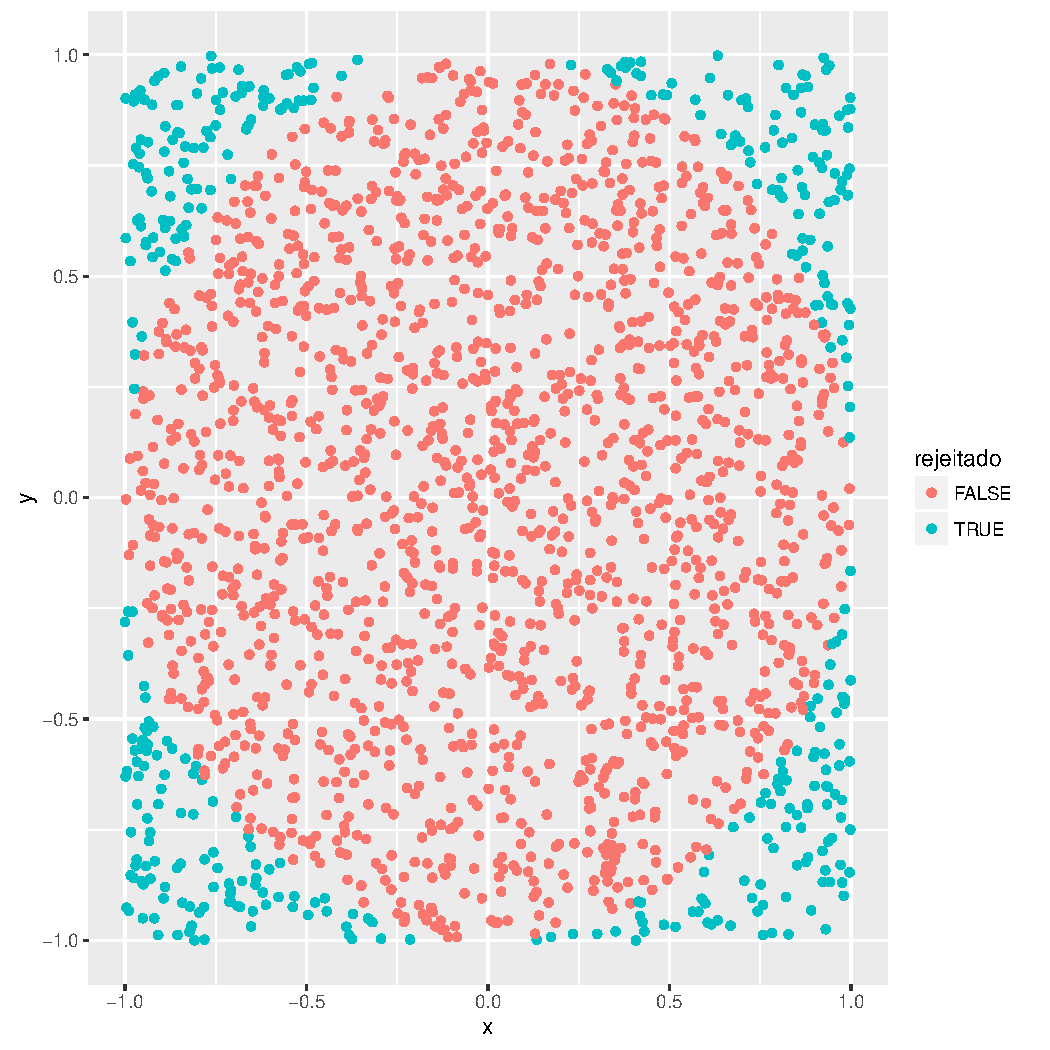
\includegraphics[scale=0.5]{chapter-computing-rejection-circle}
  \caption{Amostra de $2000$ propostas geradas pelo
  método da rejeição descrito
  no \cref{ex:rejection-circle}.}
  \label{fig:rejection-circle}
 \end{figure}
\end{example}

\begin{example}
 \label{ex:rejection-beta-2-2}
 Você deseja simular da densidade
 $f(\theta) = 6\theta(1-\theta)\I(\theta \in (0,1))$.
 Note que $f(\theta)$ é a densidade da Beta$(2,2)$.
 Podemos tomar, por exemplo,
 $\tilde{f}(\theta) = \theta(1-\theta) \I(\theta \in (0,1))$.
 Assim, $\tilde{f}(\theta) \leq 0.25 \I(\theta \in (0,1)) = 0.25 \cdot h(\theta)$,
 onde $h(\theta)$ é a densidade da
 Uniforme$(0,1)$ e $M=0.25$.
 Note que $\frac{\tilde{f}(\theta)}{M h(\theta)} = 4\theta(1-\theta)$.
 Portanto, é possível simular de $f$ pelo
 método da rejeição 
 usando o seguinte código
 \begin{verbatim}
###############################################################
## retorna: uma variável aleatória de distribuição Beta(2,2) ##
###############################################################
simula_beta_2_2_rejeicao <- function(B)
{
 amostra <- vector(mode="list", length=B)
 for(ii in 1:B)
 {
  T <- runif(1)
  while(runif(1) > 4*T*(1-T)) T <- runif(1)
  amostra[[ii]] <- T
 }
 return(amostra)
}
\end{verbatim}

 O funcionamento do algoritmo acima é ilustrado na
 \cref{fig:rejection-beta-2-2}.
 O eixo $x$ dos pontos indicam as $2000$ propostas que
 foram geradas para obter uma amostra de tamanho $1315$.
 O eixo $y$ dos pontos indicam as
 variáveis aleatórias uniformes geradas para
 determinar se as propostas eram rejeitadas.
 Dentre os pontos gerados, os vermelhos foram aceitos e
 os azuis foram rejeitados.
 Note que, como $\frac{\tilde{f}(\theta)}{h(\theta)} = 4\theta(1-\theta)$,
 $T$ era rejeitado se $U > 4T(1-T)$.
 A \cref{fig:rejection-beta-2-2} também ilustra um
 outro aspecto do método da rejeição.
 Ao combinarmos $T$ e $U$, obtemos uma
 distribuição uniforme em $[0,1]^{2}$.
 Ao remover, os pontos azuis,
 os pontos vermelhos que restam distribuem-se de
 acordo com uma distribuição Beta(2,2) no eixo $x$.
 \begin{figure}
  \centering
  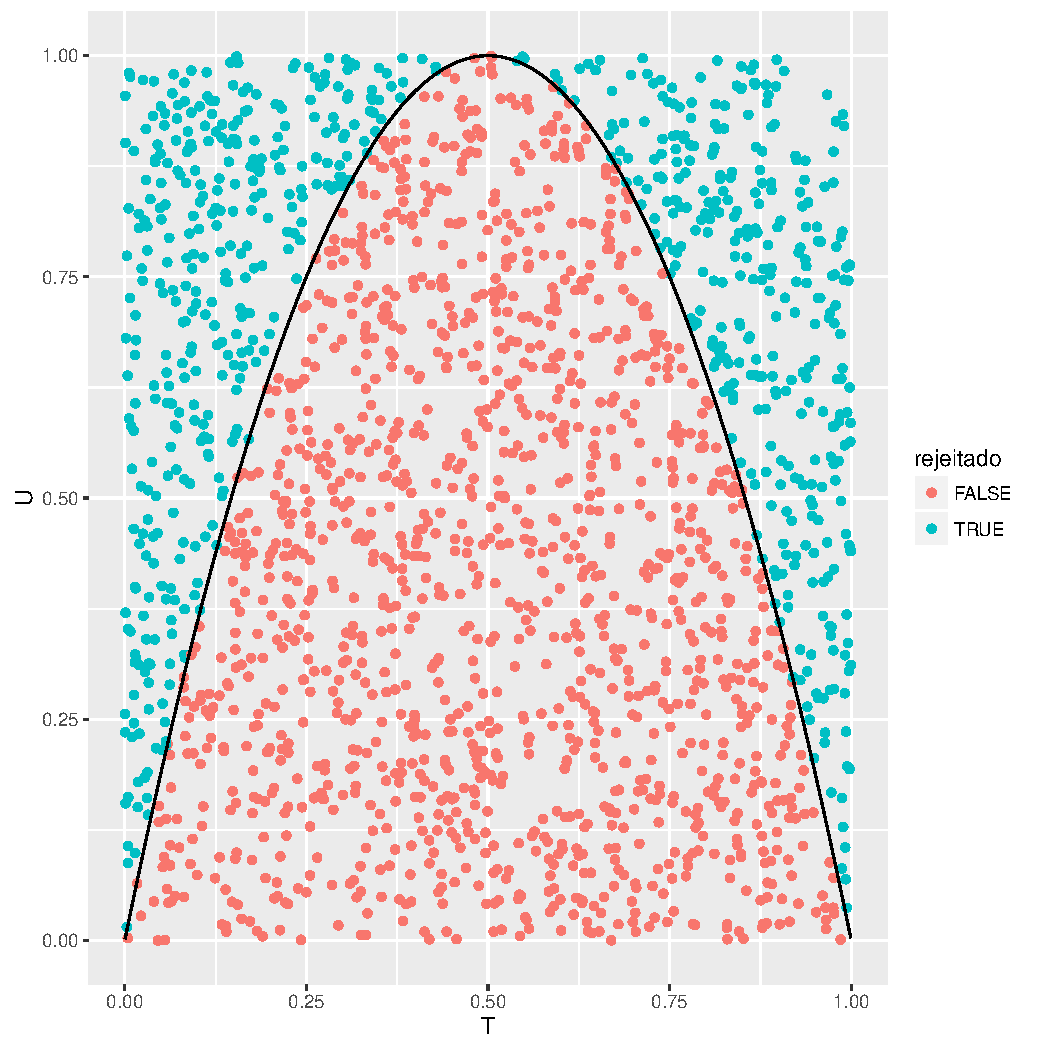
\includegraphics[scale=0.5]{chapter-computing-rejection-beta-2-2}
  \caption{Amostra de $2000$ propostas geradas pelo
  método da rejeição descrito no
  \cref{ex:rejection-beta-2-2}.}
  \label{fig:rejection-beta-2-2}
 \end{figure}
\end{example}

\begin{theorem}
 Se $\theta$ foi gerado de acordo com o
 método da rejeição usando as funções $f(\theta)$,
 $\tilde{f}(\theta)$, $h(\theta)$ e $M$
 conforme a descrição no início deste capítulo,
 então $\theta$ tem distribuição com densidade $f$.
\end{theorem}

\begin{proof}
 Considere que $N$ é o número de propostas geradas
 até a primeira aceitação, que
 $T_{1},\ldots,T_{i},\ldots$ é um conjunto de propostas e
 $U_{1},\ldots,U_{i},\ldots$ é um conjunto de uniformes.
 Note que $A_{i} = \I\left(U_{i} \leq \frac{\tilde{f}(T_{i})}{Mh(T_{i})}\right)$ são i.i.d. e
 \begin{align*}
  \P\left(U_{i} \leq
  \frac{\tilde{f}(T_{i})}
  {Mh(T_{i})}\right)
  &= \int_{-\infty}^{\infty}
  {\frac{\tilde{f}(t)}{Mh(t)} h(t) dt} \\
  &= M^{-1}\int_{-\infty}^{\infty}
  {\tilde{f}(t)dt} := p_{1}
 \end{align*}
 Portanto, como $N = \min\left(i: \I(U_{i} \leq \frac{\tilde{f}(T_{i})}{Mh(T_{i})}) =1\right)$,
 então $N \sim \text{Geométrica}(p_{1})$. Assim, para todo 
 $B \subset \mathbb{R}$,
 \begin{align*}
  \P(\theta \in B)
  &= \sum_{n}{\P(\theta \in B, N = n)} \\
  &= \sum_{n}{\P(\cap_{i=1}^{n-1}{A_{i}^{c}} \cap (A_{n} \cap T_{n} \in B))} \\
  &= \sum_{n}{\P(\cap_{i=1}^{n-1}{A_{i}^{c}})\P(A_{n} \cap T_{n} \in B)} \\
  &= \sum_{n}{(1-p_{1})^{n-1}\int_{B}{\frac{\tilde{f}(t)}{Mh(t)} h(t)dt}} \\
  &= \int_{B}{M^{-1}\tilde{f}(t)dt}\sum_{n}{(1-p_{1})^{n-1}} \\
  &= \frac{\int_{B}{M^{-1}\tilde{f}(t)dt}}{p_{1}} \\
  &= \frac{M^{-1}\int_{B}{\tilde{f}(t)dt}}{M^{-1}\int_{-\infty}^{\infty}{\tilde{f}(t)dt}} \\
  &= \int_{B}{\frac{\tilde{f}(t)}{\int_{-\infty}^{\infty}{\tilde{f}(t)dt}}dt} \\
  &= \int_{B}{f(t)dt}
 \end{align*} 
\end{proof}

\subsubsection*{Exercícios}

\begin{exercise}
 No \cref{ex:rejection-circle},
 usamos propostas de um quadrado de lado $2$
 e centro na origem.
 Poderíamos ter implementado o algoritmo da rejeição
 usando propostas de um quadrado de lado $1$?
 E de um quadrado de lado $3$?
 Esboce estas três figuras acompanhadas
 do círculo de raio $1$ e centro na origem.
 Compare as propostas sugeridas em relação à sua eficiência computacional.
\end{exercise}

\solution{\textbf{Solução}: A densidade de uma
 distribuição uniforme no quadrado de lado $1$ e
 centro na origem é,
 $h_{1}(\theta) := \I(|\theta_{1}| \leq 0.5, |\theta_{2}| \leq 0.5)$.
 Se tomarmos $f(\theta)$ como a densidade da
 distribuição uniforme no círculo de raio $1$ e
 centro na origem, então $f((1,0)) = 1$ e
 $h_{1}((1,0))$. Portanto, não existe $M > 0$ tal que
 $f((1,0)) \leq Mh_{1}((1,0))$.
														  Assim, não é possível usar o método da rejeição para  simular de $f$ a partir de $h_{1}$. 
 Por outro outro lado, defina
 $h_{2} = 4^{-1}\I(|\theta_{1}|\leq 1, |\theta_{2}|\leq 1)$ e $h_{3} = 9^{-1}\I(|\theta_{1}|\leq 1.5, |\theta_{2}|\leq 1.5)$ como as densidades dos quadrados
 de lado $2$ e $3$, e $\tilde{f}(\theta) = \I(\theta_{1}^{2}+\theta_{2}^{2} \leq 1)$.
 Note que $\tilde{f}(\theta) \leq 4 h_{2}$ e
 $\tilde{f}(\theta) \leq 9 h_{3}$.
 Assim, a probabilidade de aceitação usando
 $\tilde{f}$, $h_{2}$ e $M=4$ é dada por
 
 \begin{align*}
  \P\left(U \leq \frac{\tilde{f}(T)}{4 h_{2}(T)}\right)
  &= \int_{-\infty}^{\infty}{\frac{\tilde{f}(t)}{4 h_{2}(t)} h_{2}(t)dt} \\
  &= 4^{-1}\int_{-\infty}^{\infty}{\tilde{f}(t)dt}
  = \frac{\pi}{4}
 \end{align*}
 
 Similarmente, a probabilidade de aceitação usando
 $\tilde{f}$, $h_{3}$ e $M=9$ é $\frac{\pi}{9}$.
 Como a probabilidade de aceitação usando $h_{2}$ é
 maior do que usando $h_{3}$, o primeiro é
 mais computacionalmente eficiente.
 
 Este argumento é ilustrado pela
 \cref{fig:rejection-squares}.
 Note que a região de rejeição usando
 $h_{3}$ (azul e verde) é consideravelmente maior
 que aquela usando $h_{2}$ (verde).
 \begin{figure}
  \centering
  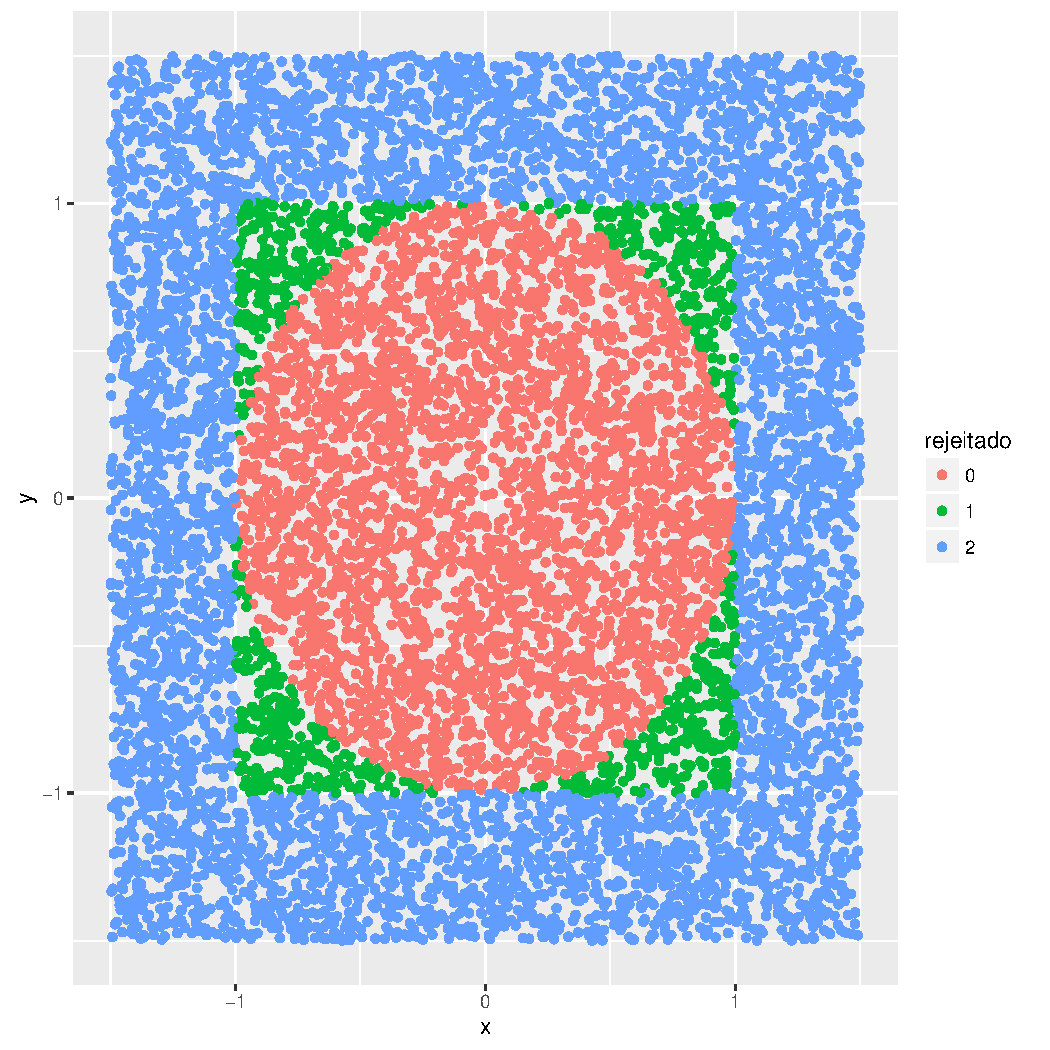
\includegraphics[scale=0.5]{chapter-computing-rejection-squares}
  \caption{Ilustração das regiões de rejeição
  para propostas de $h_{2}$ (verde) e de
  $h_{3}$ (verde e azul).}
  \label{fig:rejection-squares}
 \end{figure}
}{}

\begin{exercise}
 Escreva um código para
 simular de distribuição uniforme
 em uma esfera de raio $1$ e centro $0$.
 Use o Método de Monte Carlo para estimar
 a distância média de de um ponto amostrado à origem.
\end{exercise}

\cprotect \solution{
 \textbf{Solução}: Podemos escolher
 $\tilde{f}(\theta) = \I(\theta_{1}^{2}+\theta_{2}^{2}+\theta_{3}^{2} \leq 1)$.
 Se usarmos como propostas a uniforme no cubo de
 aresta $1$ e centro na origem, então
 $h(\theta) = 8^{-1}\I(|\theta_{i}| \leq 1, i \in \{1,2,3\})$.
 Assim, $\tilde{f}(\theta) \leq 8h(\theta)$ e
 tomamos $M=8$.
 Neste caso, $\frac{\tilde{f}(\theta)}{8h(\theta)} = \tilde{f}(\theta)$.
 Portanto, o método da rejeição pode ser implementado
 da seguinte forma
														
\begin{lstlisting}[language=R]
simula_esfera_rejeicao <- function(B) # retorna: pontos uniformemente
{                                     # da esfera de raio 1 centrada na origem.
 amostra <- vector(mode="list", length=B)
 for(ii in 1:B)
 {
  T <- runif(3,-1,1)
  while(sum(T^2) > 1) T <- runif(3,-1,1)
	amostra[[ii]] <- T
 }
 return(amostra)
}
\end{lstlisting}

Se usarmos o \cref{algo:monte_carlo}, obtemos

\begin{lstlisting}[language=R]
 B <- 10^4
 g <- function(coord) sqrt(sum(coord^2))
 monte_carlo(simula_esfera_rejeicao, B, g)
 
 estimador
 [1] 0.7484544
\end{lstlisting} 

 Note que a distância média de um ponto ao centro da
 esfera de raio $1$ é aproximadamente $0.75$.
 Assim, a distância média não é a metade do raio.
 Isto ocorre pois o volume da esfera a partir da
 metade do raio é maior do que o volume da esfera até
 a metade do raio.
}{}

\begin{exercise}
 \label{ex:circle-rejection-2}
 Escreva um código para
 simular de uma distribuição uniforme 
 em um círculo de raio $r$ e centro $c$.
 Qual é a relação entre o raio do círculo e a 
 distância média de um ponto amostrado ao seu centro?
 Exiba uma figura que ilustre essa relação.
\end{exercise}

\cprotect \solution{\textbf{Solução}: 
 Existem ao menos duas soluções para este problema.
 A primeira utiliza a simulação da distribuição uniforme
 no círculo de raio $1$ e centro na origem
 (\cref{ex:rejection-circle})
 para obter distribuições uniformes em outros círculos.
 Note que, se $\theta$ tem distribuição uniforme
 no círculo de raio $1$ e centro na origem,
 então $r \theta + c$ tem distribuição
 uniforme no círculo de raio $r$ e centro $c$.

 A segunda solução consiste em simular diretamente
 da distribuição uniforme no círculo de raio $r$ e
 centro $c$. Esta distribuição tem densidade
 $f(\theta) = \frac{1}{\pi r^{2}}\I((\theta_{1}-c_{1})^{2}+(\theta_{2}-c_{2})^{2} \leq r^{2})$.
 Portanto, podemos tomar
 $\tilde{f}(\theta) = \I((\theta_{1}-c_{1})^{2}+(\theta_{2}-c_{2})^{2} \leq r^{2})$.
 Para simular desta distribuição, podemos tomar o
 quadrado de lado $2r$ e centro em $c$.
 Assim, $h(\theta) = (2r)^{-2}\I(|\theta_{1}-c_{1}| \leq r, |\theta_{2}-c_{2}| \leq r)$.
 Portanto, $\tilde{f}(\theta) \leq (2r)^{2}h(\theta)$ e
 obtemos $\frac{\tilde{f}(\theta)}{(2r)^{2}h(\theta)} = \tilde{f}(\theta)$.
 Assim, é possível simular de $f$ pelo
 método da rejeição usando o seguinte código

 \begin{lstlisting}[language=R]
simula_circulo_rejeicao <- function(B, centro, raio)
{
 amostra <- vector(mode="list", length=B)
 for(ii in 1:B)
 {
  T <- runif(2,-raio,raio)+centro
  while(sum(((T-centro)/raio)^2) > 1) T <- runif(2,-raio,raio)+centro
  amostra[[ii]] <- T
 }
 return(amostra)
}
 \end{lstlisting}

 Podemos obter estimadores da distâncias ao
 centro do círculo e exibi-los graficamente usando o
 seguinte código:

 \begin{lstlisting}[language=R]
 raios <- 1:10
 estimadores <- rep(NA, length(raios))
 g <- function(coord) sqrt(sum(coord^2))
 for(ii in 1:length(raios)) 
 {
  estimadores[ii] <- monte_carlo(simula_circulo_rejeicao, 10^3, g, 
                                 c(0,0), raios[ii])[["estimador"]]
 }
 dados <- data.frame(raio=raios, distancia=estimadores)
 ggplot(data=dados, aes(x=raio, y=distancia))+
 geom_point()+
 geom_smooth(method='lm',formula=y~x)
 \end{lstlisting}

O resultado é exibido na
\cref{fig:circle-rejection-2}.

\begin{figure}
 \centering
 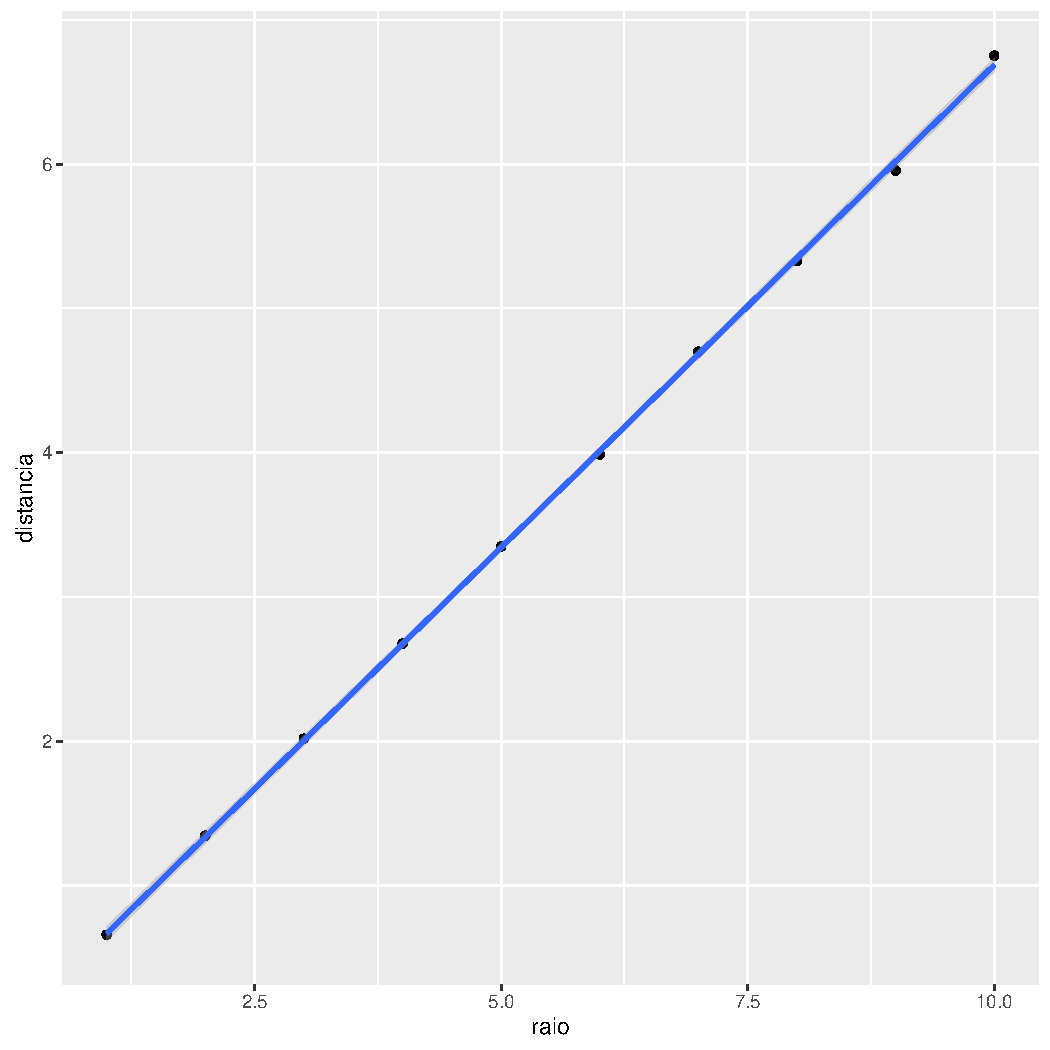
\includegraphics[scale=0.3]{chapter-computing-circle-distance}
 \caption{Variação linear da distância ao centro de
 acordo com o raio (\cref{ex:circle-rejection-2}).}
 \label{fig:circle-rejection-2}
\end{figure}
}{}

\begin{exercise}
 \label{ex:rejection-beta-a-b}
 Escreva código para
 simular de uma $\text{Beta}(a,b)$
 a partir de uma $\text{Uniforme}(0,1)$.
 Estime a média da $\text{Beta}(a,b)$ pelo
 método de Monte Carlo.
 Compare as taxas de rejeição do algoritmo proposto
 para alguns valores de $a$ e de $b$.
 Qual é a relação entre esses valores e
 a eficiência computacional do algoritmo proposto?
\end{exercise}

\cprotect \solution{\textbf{Solução}:
 O problema determina que
 $h(\theta) = \I(0 \leq \theta \leq 1)$.
 Podemos tomar $f(\theta) = \tilde{f}(\theta) = dbeta(\theta,a,b)$.
 Note que a moda da Beta$(a,b)$ é
 $\frac{a-1}{a+b-2}$. Portanto,
 $\tilde{f}(\theta) \leq \tilde{f}\left(\frac{a-1}{a+b-2}\right)h(\theta)$.
 Assim, as condições na amostragem por rejeição
 estão satisfeitas tomando
 $M= \tilde{f}\left(\frac{a-1}{a+b-2}\right)$.
 Portanto, podemos simular da Beta$(a,b)$ da
 seguinte forma
 \begin{lstlisting}[language=R]
simula_beta_rejeicao <- function(B,alpha,beta)
{
 M <- dbeta((alpha-1)/(alpha+beta-2),alpha,beta)
 amostra <- vector(mode="list", length=B)
 for(ii in 1:B)
 {
  T <- runif(1,0,1)
	rejeicoes <- 0
  while(runif(1,0,1) > dbeta(T,alpha,beta)/M) 
	{
	 T <- runif(1,0,1)
   rejeicoes <- rejeicoes+1
	}
	amostra[[ii]] <- c(T, rejeicoes)
 }
 return(amostra)
}
 \end{lstlisting} 

 Para entender de que forma o número de rejeições se
 comporta de acordo com $a$ e $b$, 
 geraremos amostradores para os casos em que $a=b$,
 para diversos valores de $a$ entre $2$ e $10$.
 O código está exibido abaixo.

 \begin{lstlisting}[language=R]
rejeicoes <- function(x) x[2]
param <- 2:10 
estimadores <- rep(NA, length(param))
for(ii in 1:length(param))
{
 estimadores[ii] <- monte_carlo(simula_beta_rejeicao, 10^4, rejeicoes, 
                                param[ii], param[ii])[["estimador"]]
}
dados <- data.frame(parametros=param, rejeicoes=estimadores)
ggplot(data=dados, aes(x=parametros, y=rejeicoes))+
geom_point()+
geom_smooth(method='lm',formula=y~x)
 \end{lstlisting}

 \begin{figure}
  \centering
  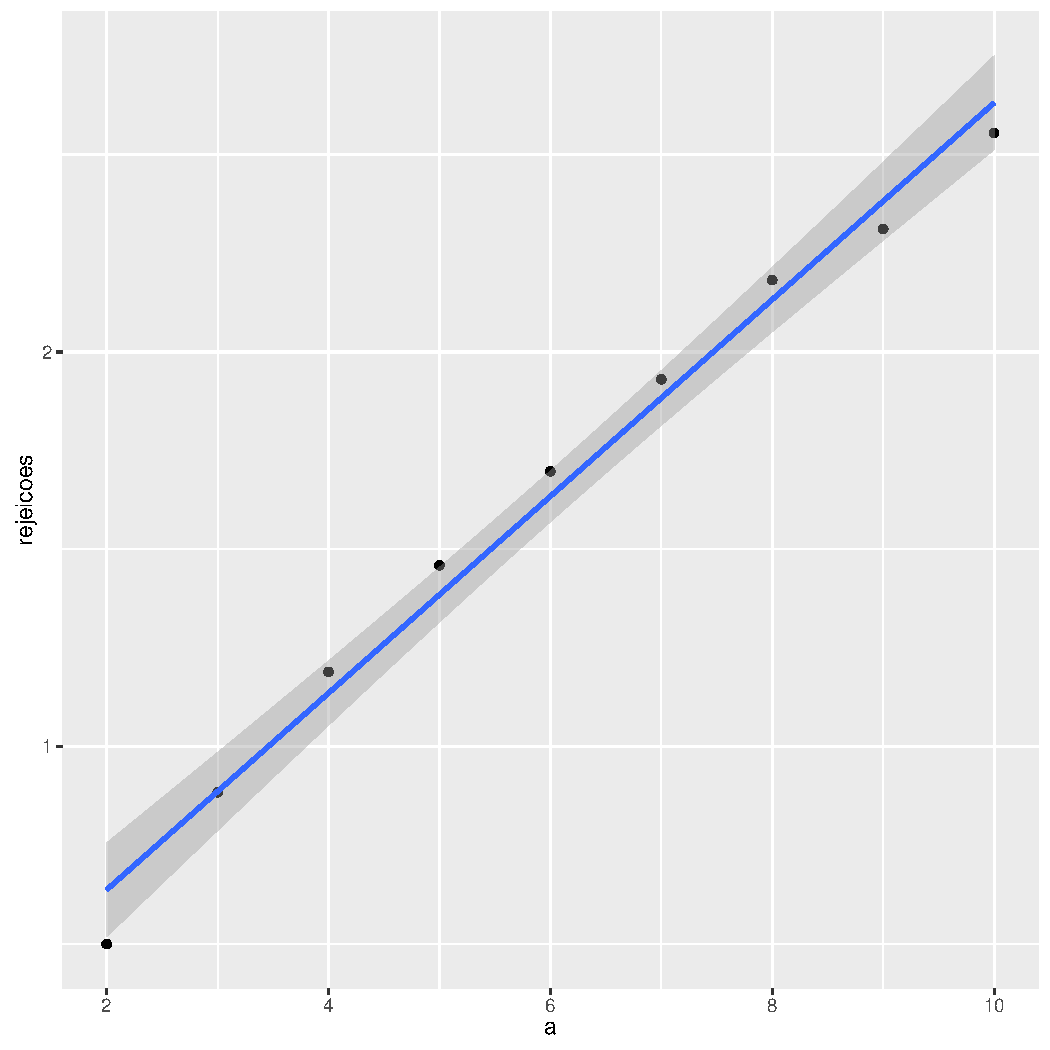
\includegraphics[scale=0.3]{chapter-computing-beta-rejections}
  \caption{Variação da taxa de rejeição
  de acordo com o valor de $a$
  (\cref{ex:rejection-beta-a-b}).}
  \label{fig:rejection-beta-a-b-1}
 \end{figure}

 A \cref{fig:rejection-beta-a-b-1} mostra que,
 quanto maiores os valores de $a$ e $b$, 
 maior a taxa de rejeição. 
 Isto ocorre pois a distribuição da Beta(a,b) 
 fica mais ``diferente'' da distribuição Uniforme(0,1)
 à medida que o valor de $a$ e $b$ aumentam.
 Este fato é ilustrado na
 \cref{fig:rejection-beta-a-b-2}.

 \begin{figure}
  \centering
  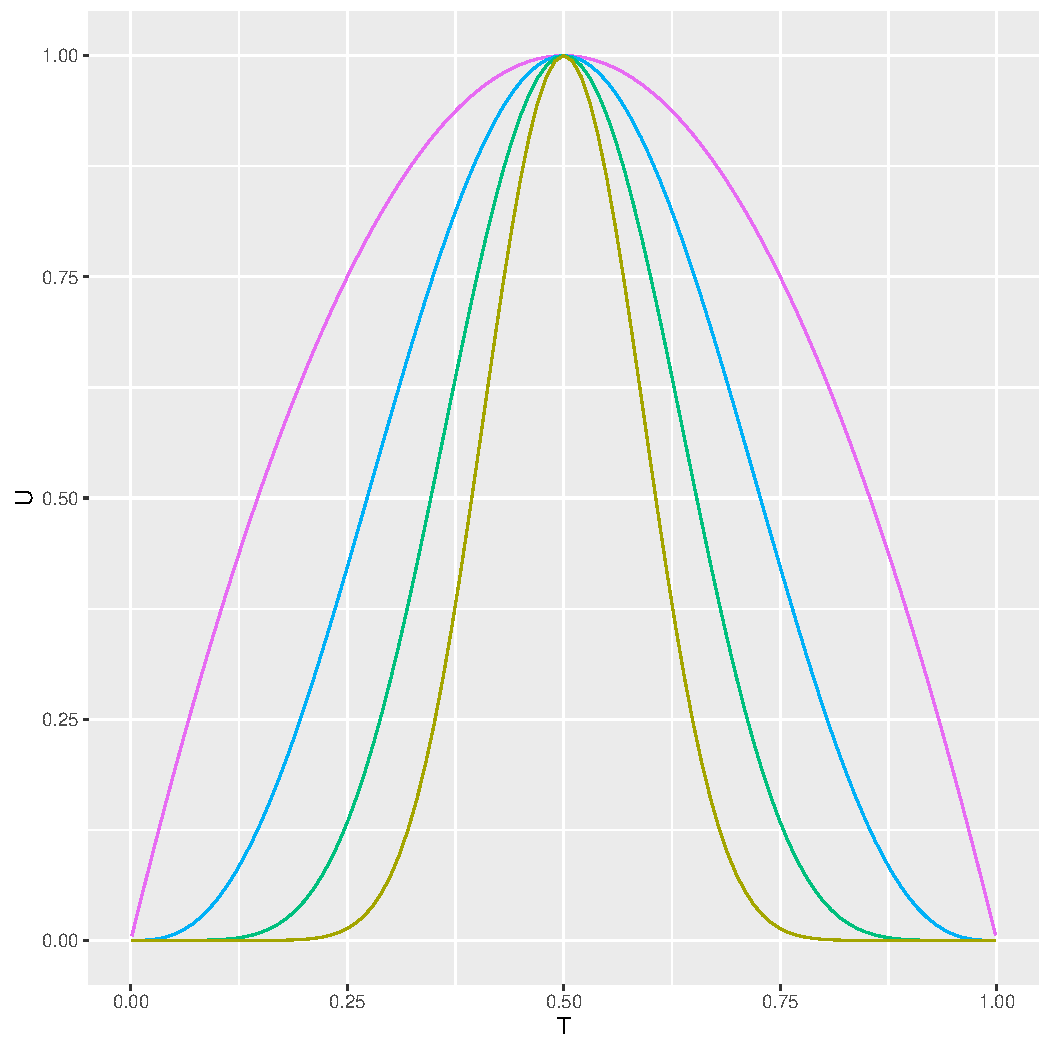
\includegraphics[scale=0.5]{chapter-computing-rejection-beta-a-b}
  \caption{Ilustração das regiões de rejeição
  para a Beta(2,2) (roxo), a Beta(4,4) (azul),
  a Beta(8,8) (verde) e a Beta(16,16) (marrom).}
  \label{fig:rejection-beta-a-b-2}
 \end{figure}
}{}

\begin{exercise}
 Sob quais condições é possível usar
 o método da rejeição para simular de
 uma $\text{Beta}(a,b)$ a partir de uma
 $\text{Beta}(a^{*},b^{*})$?
\end{exercise}

\cprotect \solution{\textbf{Solução}:
 Se $f(\theta) = dbeta(a,b)$ e
 $h(\theta) = dbeta(a^{*},b^{*})$, então
 \begin{align*}
  \frac{f(\theta)}{h(\theta)}
  &= \frac{Beta^{-1}(a,b)\theta^{a-1}(1-\theta)^{b-1}}{Beta^{-1}(a^{*},b^{*})\theta^{a^{*}-1}(1-\theta)^{b^{*}-1}} \\
  &= \frac{Beta(a^{*},b^{*})}
  {Beta(a,b)} \theta^{a-a^{*}}(1-\theta)^{b-b^{*}}
 \end{align*}
 Note que, se $a < a^{*}$, então
 $\frac{f(\theta)}{h(\theta)}$ pode ser
 arbitrariamente grande tomando-se $\theta \approx 0$.
 Similarmente, se $b < b^{*}$, então
 $\frac{f(\theta)}{h(\theta)}$ pode ser
 arbitrariamente grande tomando-se $\theta \approx 1$.
 Nestes casos, não existe $M$ tal que
 $f(\theta) \leq Mh(\theta)$.
 Portanto, se $a< a^{*}$ ou $b < b^{*}$,
 então não é possível amostrar de uma Beta$(a,b)$ 
 a partir de uma Beta$(a^{*},b^{*})$.

 Contudo, se $a>a^{*}$ e $b>b^{*}$,
 então $\frac{f(\theta)}{h(\theta)}$ é
 proporcional à densidade de uma
 Beta$(a-a^{*}+1,b-b^{*}+1)$.
 Portanto, $\frac{f(\theta)}{h(\theta)}$ tem
 seu valor maximizado em
 $\theta = \frac{a-a^{*}}{a-a^{*}+b-b^{*}}$.
 Assim, obtemos,
 \begin{align*}
  \frac{f(\theta)}{h(\theta)}
  &\leq \frac{Beta(a^{*},b^{*})}{Beta(a,b)} \left(\frac{a-a^{*}}{a-a^{*}+b-b^{*}}\right)^{a-a^{*}}\left(1-\frac{a-a^{*}}{a-a^{*}+b-b^{*}}\right)^{b-b^{*}} \\
  f(\theta) &\leq \frac{Beta(a^{*},b^{*})}{Beta(a,b)} \left(\frac{a-a^{*}}{a-a^{*}+b-b^{*}}\right)^{a-a^{*}}\left(1-\frac{a-a^{*}}{a-a^{*}+b-b^{*}}\right)^{b-b^{*}} h(\theta)
 \end{align*}
 Portanto, podemos tomar $\tilde{f}(\theta)=f(\theta)$ e
 $M=\frac{Beta(a^{*},b^{*})}{Beta(a,b)} \left(\frac{a-a^{*}}{a-a^{*}+b-b^{*}}\right)^{a-a^{*}}\left(1-\frac{a-a^{*}}{a-a^{*}+b-b^{*}}\right)^{b-b^{*}}$.
 
 Assim, obtemos o código:

 \begin{lstlisting}[language=R]
# retorna uma beta(a1, b1) pelo metodo da rejeicao
# por meio de uma beta(a2,b2)
simula_beta_via_beta <- function(B,a1,b1,a2,b2) {
 M <- ((a1-a2)/(a1-a2+b1-b2))^(a1-a2)*(1-(a1-a2)/(a1-a2+b1-b2))^(b1-b2)
 amostra <- vector(mode="list", length=B)
 for(ii in 1:B) {
  T <- rbeta(1,a2,b2)
  while(runif(1) > T^(a1-a2)*(1-T)^(b1-b2)/M)  T <- rbeta(1,a2,b2)
  amostra[[ii]] <- T
 }
 return(amostra)
}
 \end{lstlisting}
}{}

\begin{exercise}
 Sob quais condições é possível usar
 o método da rejeição para simular de uma
 $\text{Gama}(a,b)$ a partir de uma
 $\text{Exponencial}(c)$? Escreva o
 código para realizar esta simulação. 
\end{exercise}

